\documentclass[11pt]{article}

\usepackage[margin=1in]{geometry}
\usepackage{amsmath,amssymb}
\usepackage{booktabs}
\usepackage{array}
\usepackage{hyperref}
\usepackage{xcolor}
\usepackage{tikz}
\usepackage{pgfplots}
\pgfplotsset{compat=1.18}
\usetikzlibrary{arrows.meta,positioning,shapes.geometric,fit}

\title{AMM Dynamic Fee Strategy: Equation-Centric Technical Report\\
\large Consolidated from \texttt{Strategy.sol} and \texttt{yq-v2} analyses}
\author{}
\date{2026-02-10}

\begin{document}
\maketitle
\tableofcontents
\newpage

\section{Purpose and Scope}
This report gives a deep, equation-first explanation of the strategy implementation and proposed extensions, consolidating:
\begin{itemize}
    \item \texttt{research/strategy-sol-math-report.md}
    \item \texttt{research/yq-v2-math-report.md}
\end{itemize}

It focuses on:
\begin{enumerate}
    \item precise variable definitions,
    \item exact update equations and control flow,
    \item mathematical interpretation of each term,
    \item ranked improvement suggestions with equation forms.
\end{enumerate}

\section{Notation and Core Simulator Math}
\subsection{Symbols}
\begin{center}
\begin{tabular}{>{\ttfamily}p{2.6cm} p{10.5cm}}
\toprule
Symbol & Meaning \\
\midrule
$x, y$ & AMM reserves of token X and token Y \\
$k$ & Constant-product invariant, $k = xy$ \\
$s$ & AMM spot price, $s = y/x$ (Y per X) \\
$f$ & Fee (WAD-scaled in Solidity, decimal in simulator math) \\
$\gamma$ & Fee multiplier, $\gamma = 1-f$ \\
$p$ & External fair price from GBM \\
$\hat p$ & Internal fair-price estimate (\texttt{pHat}) \\
$\hat \sigma$ & Volatility estimate (\texttt{sigmaHat}) \\
$\hat \lambda$ & Trade-arrival estimate (\texttt{lambdaHat}) \\
$\hat q$ & Trade-size estimate (\texttt{sizeHat}) \\
$\hat \tau$ & Toxicity EMA (\texttt{toxEma}, denoted toxSignal) \\
$a$ & Activity EMA (\texttt{actEma}) \\
$d$ & Direction state (\texttt{dirState}), centered at $1$ (WAD) \\
\bottomrule
\end{tabular}
\end{center}

\subsection{Objective}
The scoring objective can be viewed as:
\begin{equation}
\mathbb{E}[\text{Edge}] = \mathbb{E}[\text{Retail Edge}] - \mathbb{E}[\text{Arbitrage Loss}]
\end{equation}

This creates a strict trade-off:
\begin{itemize}
    \item higher fees reduce arbitrage intensity,
    \item but higher fees reduce routed retail flow.
\end{itemize}

\subsection{AMM and fee-on-input model}
\begin{equation}
k = xy,\qquad s = \frac{y}{x},\qquad \gamma = 1-f.
\end{equation}

When fees are taken on input, only a fraction $\gamma$ of input moves reserves.

\subsection{Arbitrage optimal trade sizes}
For fair price $p$, reserves $(x,y)$:
\begin{align}
\text{If } s < p:\quad &\Delta x_{\text{out}}^\star = x - \sqrt{\frac{k}{\gamma p}}, \\
\text{If } s > p:\quad &\Delta x_{\text{in}}^\star = \frac{\sqrt{\frac{k\gamma}{p}} - x}{\gamma}.
\end{align}

These equations explain why higher fees can create larger stale-price bands.

\subsection{Retail routing split (two AMMs)}
For buy-side total order size $Y$, AMM $i \in \{1,2\}$:
\begin{equation}
A_i = \sqrt{x_i \gamma_i y_i},\qquad r=\frac{A_1}{A_2},
\end{equation}
\begin{equation}
\Delta y_1 = \frac{r\left(y_2 + \gamma_2 Y\right)-y_1}{\gamma_1 + r\gamma_2},
\qquad
\Delta y_2 = Y - \Delta y_1.
\end{equation}

This split is nonlinear in fees; small fee changes can produce large flow-share changes.

\subsection{Plot: flow share vs own fee}
Assumptions for this plot:
\begin{itemize}
    \item equal starting reserves ($x_1=x_2=100$, $y_1=y_2=10000$),
    \item competitor fixed at $30$ bps,
    \item order size $Y=20$ (near mean retail size).
\end{itemize}

\begin{center}
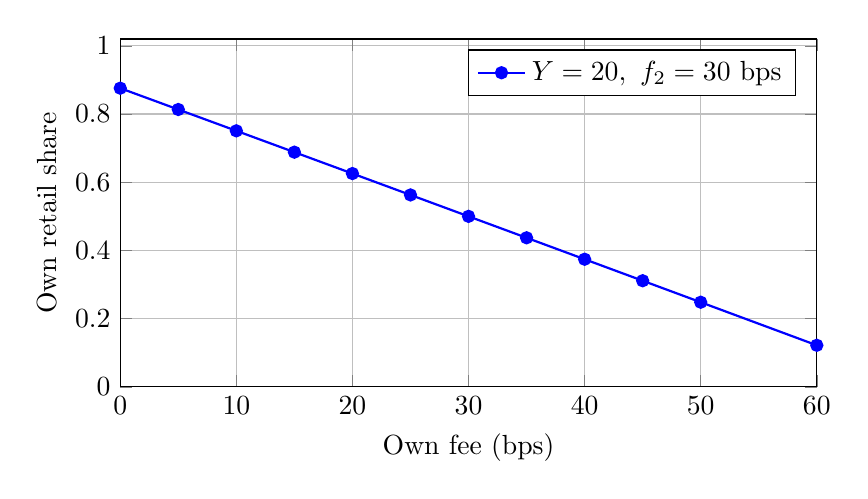
\begin{tikzpicture}
\begin{axis}[
    width=0.86\textwidth,
    height=6cm,
    xlabel={Own fee (bps)},
    ylabel={Own retail share},
    ymin=0, ymax=1.02,
    xmin=0, xmax=60,
    grid=both,
    legend pos=north east
]
\addplot[blue,thick,mark=*] coordinates {
(0,0.875753)
(5,0.813284)
(10,0.750753)
(15,0.688159)
(20,0.625502)
(25,0.562783)
(30,0.500000)
(35,0.437154)
(40,0.374246)
(45,0.311274)
(50,0.248239)
(60,0.121978)
};
\addlegendentry{$Y=20,\ f_2=30\text{ bps}$}
\end{axis}
\end{tikzpicture}
\end{center}

\noindent
Interpretation: even moving from $0$ to $10$ bps has a large share impact for typical trade sizes.

\subsection{Plot: share vs order size (cannot always capture 100\%)}
\begin{center}
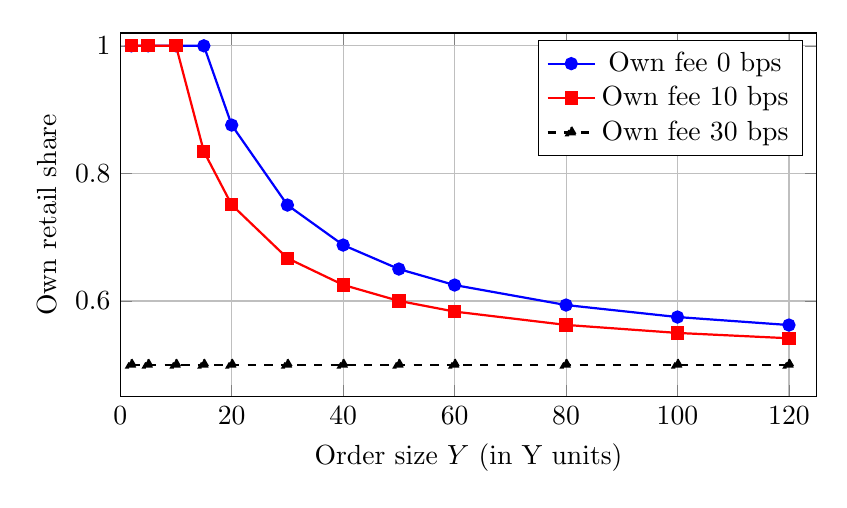
\begin{tikzpicture}
\begin{axis}[
    width=0.86\textwidth,
    height=6.2cm,
    xlabel={Order size $Y$ (in Y units)},
    ylabel={Own retail share},
    ymin=0.45, ymax=1.02,
    xmin=0, xmax=125,
    grid=both,
    legend style={at={(0.98,0.98)},anchor=north east}
]
\addplot[blue,thick,mark=*] coordinates {
(2,1.0) (5,1.0) (10,1.0) (15,1.0) (20,0.875753) (30,0.750377)
(40,0.687689) (50,0.650076) (60,0.625) (80,0.593656) (100,0.574850) (120,0.562312)
};
\addlegendentry{Own fee 0 bps}

\addplot[red,thick,mark=square*] coordinates {
(2,1.0) (5,1.0) (10,1.0) (15,0.834420) (20,0.750753) (30,0.667085)
(40,0.625251) (50,0.600151) (60,0.583417) (80,0.562500) (100,0.549950) (120,0.541583)
};
\addlegendentry{Own fee 10 bps}

\addplot[black,thick,dashed,mark=triangle*] coordinates {
(2,0.5) (5,0.5) (10,0.5) (15,0.5) (20,0.5) (30,0.5)
(40,0.5) (50,0.5) (60,0.5) (80,0.5) (100,0.5) (120,0.5)
};
\addlegendentry{Own fee 30 bps}
\end{axis}
\end{tikzpicture}
\end{center}

\noindent
Interpretation: with equal reserves and a 30 bps competitor, setting fee below 30 bps improves share but does not guarantee full capture for larger orders.

\section{Deep Equation Walkthrough of \texttt{Strategy.sol}}
\subsection{State vector and initialization}
Define the latent-state vector:
\begin{equation}
\mathbf{z}_t = 
\begin{bmatrix}
d_t,\ a_t,\ \hat p_t,\ \hat \sigma_t,\ \hat \lambda_t,\ \hat q_t,\ \hat \tau_t,\ n_t
\end{bmatrix},
\end{equation}
where $n_t$ is within-step trade count.

Initialization sets:
\begin{align}
d_0 &= 1,\\
\hat p_0 &= \frac{y_0}{x_0},\\
\hat \sigma_0,\hat \lambda_0,\hat q_0 &>0\ \text{(nonzero priors for stability)}.
\end{align}

\subsection{Step-boundary decay and arrival update}
Let $\Delta t$ be elapsed steps since last observed timestamp.
State decays are:
\begin{align}
d_t &\leftarrow 1 + (d_t-1)\cdot \delta_d^{\Delta t} \quad\text{(or symmetric form below 1)},\\
a_t &\leftarrow a_t\cdot \delta_a^{\Delta t},\\
\hat q_t &\leftarrow \hat q_t\cdot \delta_q^{\Delta t},\\
\hat \tau_t &\leftarrow \hat \tau_t\cdot \delta_\tau^{\Delta t}.
\end{align}

Arrival-rate update from step count:
\begin{equation}
\lambda_{\text{inst}} = \min\!\left(\frac{n_{t-1}}{\Delta t},\ \lambda_{\max}\right),
\end{equation}
\begin{equation}
\hat \lambda_t \leftarrow \rho_\lambda \hat \lambda_t + (1-\rho_\lambda)\lambda_{\text{inst}}.
\end{equation}

\subsection{First-in-step indicator}
\begin{equation}
\text{isNewStep} = \mathbf{1}\{timestamp_t > timestamp_{t-1}\},
\end{equation}
\begin{equation}
\text{firstInStep} = \mathbf{1}\{n_t=0\}\ \text{after new-step reset}.
\end{equation}

This indicator is central for selective transition logic.

\subsection{Implied price from executed trade side}
Using previous quoted fee $f_{\text{used}}$:
\begin{equation}
\gamma_{\text{used}} = 1-f_{\text{used}},
\end{equation}
\begin{equation}
p^{\text{impl}}_t=
\begin{cases}
s_t\gamma_{\text{used}}, & \text{if AMM buys X},\\[2mm]
s_t/\gamma_{\text{used}}, & \text{if AMM sells X}.
\end{cases}
\end{equation}

Relative deviation:
\begin{equation}
r_t = \frac{|p^{\text{impl}}_t-\hat p_t|}{\hat p_t}.
\end{equation}

\subsection{Adaptive gate and state updates}
Shock gate:
\begin{equation}
g_t = \max\left(c_g\hat \sigma_t,\ g_{\min}\right).
\end{equation}

Only if $r_t \le g_t$, update $\hat p$:
\begin{equation}
\hat p_t \leftarrow (1-\alpha_t)\hat p_t + \alpha_t p^{\text{impl}}_t,
\quad
\alpha_t=
\begin{cases}
\alpha_{\text{step}}, & \text{firstInStep},\\
\alpha_{\text{retail}}, & \text{otherwise}.
\end{cases}
\end{equation}

First-trade sigma update:
\begin{equation}
\hat \sigma_t \leftarrow \rho_\sigma \hat \sigma_t + (1-\rho_\sigma)\min(r_t,r_{\max}).
\end{equation}

\subsection{Flow, direction, activity, and size}
Trade intensity proxy:
\begin{equation}
q_t = \min\!\left(\frac{\text{amountY}_t}{\text{reserveY}_t},\ q_{\max}\right).
\end{equation}

If $q_t$ exceeds signal threshold:
\begin{align}
\Delta d_t &= \min(c_d q_t,\ \Delta d_{\max}),\\
d_t &\leftarrow 
\begin{cases}
\min(2,\ d_t+\Delta d_t), & \text{if AMM buys X},\\
\max(0,\ d_t-\Delta d_t), & \text{otherwise},
\end{cases}\\
a_t &\leftarrow \rho_a a_t + (1-\rho_a)q_t,\\
\hat q_t &\leftarrow \min\!\left(1,\ \rho_q \hat q_t + (1-\rho_q)q_t\right).
\end{align}

\subsection{Toxicity}
\begin{equation}
\tau_t^{\text{raw}} = \frac{|s_t-\hat p_t|}{\hat p_t},
\qquad
\tau_t = \min(\tau_t^{\text{raw}},\tau_{\max}),
\end{equation}
\begin{equation}
\hat \tau_t \leftarrow \rho_{\tau b}\hat \tau_t + (1-\rho_{\tau b})\tau_t.
\end{equation}

\subsection{Mid-fee decomposition}
Flow-size interaction:
\begin{equation}
\phi_t = \hat \lambda_t \hat q_t.
\end{equation}

Base:
\begin{equation}
f_t^{\text{base}} = f_0 + c_\sigma \hat \sigma_t + c_\lambda \hat \lambda_t + c_\phi \phi_t.
\end{equation}

Symmetric widening:
\begin{equation}
f_t^{\text{mid}} = f_t^{\text{base}}
+ c_1\hat\tau_t
+ c_2\hat\tau_t^2
+ c_3\hat\tau_t^3
+ c_a a_t
+ c_{\sigma\tau}\hat\sigma_t\hat\tau_t.
\end{equation}

\subsection{Directional and stale-sign asymmetry}
Direction deviation:
\begin{equation}
\delta_t = |d_t-1|.
\end{equation}

Skew magnitude:
\begin{equation}
\kappa_t = c_\delta\delta_t + c_{\delta\tau}\delta_t\hat\tau_t.
\end{equation}

Directional split:
\begin{equation}
(f_t^{bid},f_t^{ask})=
\begin{cases}
(f_t^{mid}+\kappa_t,\ \max(f_t^{mid}-\kappa_t,0)), & d_t\ge 1,\\
(\max(f_t^{mid}-\kappa_t,0),\ f_t^{mid}+\kappa_t), & d_t<1.
\end{cases}
\end{equation}

Stale-sign shift (protect side up, attract side down):
\begin{equation}
\Delta_s = c_s\hat\tau_t,\qquad
\Delta_a = \eta\Delta_s,\quad \eta>1.
\end{equation}

\subsection{Trade-aligned toxicity boost}
If trade side aligns with stale sign, add:
\begin{equation}
\Delta_{\text{trade}} = c_{\text{trade}}\ q_t
\end{equation}
to the likely-protect side.

\subsection{Tail compression}
For knee $k_f$ and slope $\beta\in(0,1)$:
\begin{equation}
\mathcal{C}(f;\beta)=
\begin{cases}
f, & f\le k_f,\\
k_f+\beta(f-k_f), & f>k_f.
\end{cases}
\end{equation}

This compresses high-end fee tails while preserving monotonicity.

\subsection{Control-flow diagram}
\begin{center}
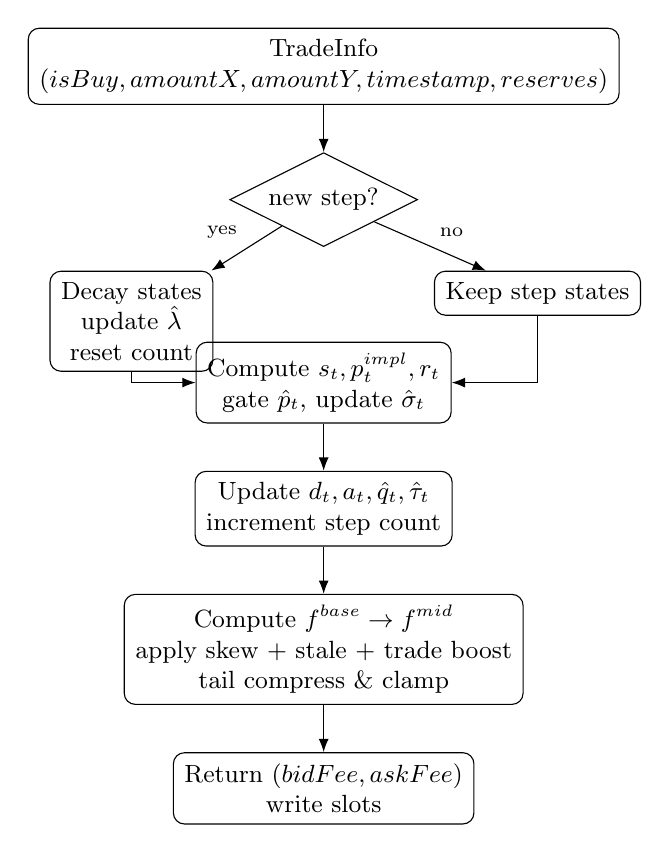
\begin{tikzpicture}[
    node distance=6mm and 8mm,
    box/.style={draw,rounded corners,align=center,inner sep=4pt,font=\small},
    decision/.style={diamond,draw,align=center,inner sep=2pt,font=\small,aspect=2}
]
\node[box] (in) {TradeInfo\\$(isBuy,amountX,amountY,timestamp,reserves)$};
\node[decision,below=of in] (new) {new step?};
\node[box,below left=of new] (decay) {Decay states\\update $\hat\lambda$\\reset count};
\node[box,below right=of new] (nostep) {Keep step states};
\node[box,below=12mm of new] (price) {Compute $s_t,p^{impl}_t,r_t$\\gate $\hat p_t$, update $\hat\sigma_t$};
\node[box,below=of price] (flow) {Update $d_t,a_t,\hat q_t,\hat\tau_t$\\increment step count};
\node[box,below=of flow] (fee) {Compute $f^{base}\to f^{mid}$\\apply skew + stale + trade boost\\tail compress \& clamp};
\node[box,below=of fee] (out) {Return $(bidFee,askFee)$\\write slots};
\draw[-{Latex}] (in) -- (new);
\draw[-{Latex}] (new) -- node[above left,font=\scriptsize]{yes} (decay);
\draw[-{Latex}] (new) -- node[above right,font=\scriptsize]{no} (nostep);
\draw[-{Latex}] (decay) |- (price);
\draw[-{Latex}] (nostep) |- (price);
\draw[-{Latex}] (price) -- (flow);
\draw[-{Latex}] (flow) -- (fee);
\draw[-{Latex}] (fee) -- (out);
\end{tikzpicture}
\end{center}

\section{yq-v2 Extension: Sigma Momentum}
`yq-v2` adds previous-step sigma memory and a momentum term:
\begin{equation}
\Delta \hat \sigma_t = \max(\hat \sigma_t - \hat \sigma_{t-1},0),
\end{equation}
\begin{equation}
f^{mid}_t \leftarrow f^{mid}_t + c_m \Delta\hat\sigma_t,\qquad c_m=0.20.
\end{equation}

Interpretation:
\begin{itemize}
    \item catches volatility acceleration before the sigma EMA alone fully rises,
    \item should be small and selective to avoid retail-flow damage.
\end{itemize}

\section{Consolidated Suggestions with Ratings}
\subsection{Rating scale}
\begin{itemize}
    \item 10: strongest mathematical fit for this simulator and architecture.
    \item 1: weak fit or structurally misaligned.
\end{itemize}

\begin{center}
\begin{tabular}{p{4.4cm} p{5.8cm} c p{3.0cm}}
\toprule
Suggestion & Equation form & Score & Core rationale \\
\midrule
One-shot transition boost & $1_{\text{firstInStep}} \cdot c \cdot [\Delta\hat\sigma]_+$ & 9/10 & avoids repeated same-step overtaxing \\
Relative sigma surprise & $c\cdot\left[\frac{[\Delta\hat\sigma]_+}{\max(\hat\sigma_{t-1},\epsilon)}-\theta\right]_+$ & 8/10 & scale-invariant trigger \\
Toxicity-gated transition & $c\cdot trigger \cdot \min(1,\hat\tau/\tau^\star)$ & 8/10 & protect only when stale risk is high \\
Calm attract anchor & if $\hat\tau<\tau_{low}$ and $a<a_{low}$ then $f_{attract}\le f_N+b$ & 8/10 & preserve routing share \\
Regime + hysteresis & switch by $T_{on},T_{off}$ with $T_{off}<T_{on}$ & 7/10 & stable mode switching \\
Reserve asymmetric penalty & signed inventory term with side-selective penalty & 6/10 & plausible but tune-sensitive \\
Intra-step escalation & repeated within-step widening & 2/10 & usually taxes retail too much \\
\bottomrule
\end{tabular}
\end{center}

\subsection{Plot: relative-sigma surprise trigger}
Define:
\begin{equation}
u = \frac{[\Delta\hat\sigma]_+}{\max(\hat\sigma_{t-1},\epsilon)},\qquad
T(u)=\max(u-\theta,0).
\end{equation}

\begin{center}
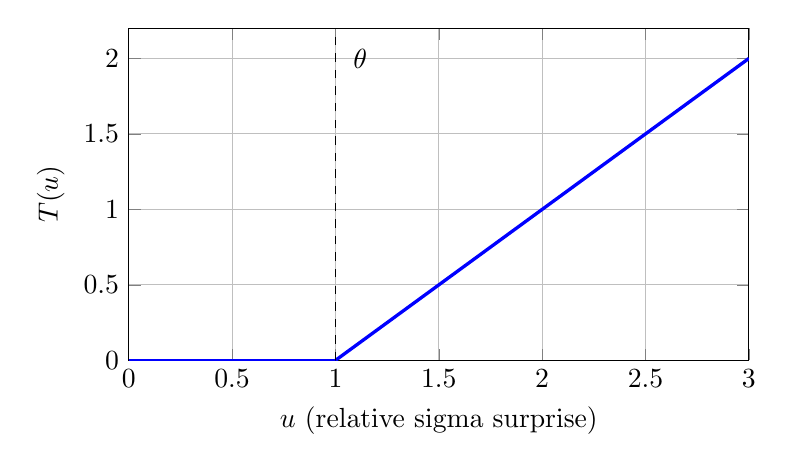
\begin{tikzpicture}
\begin{axis}[
    width=0.78\textwidth,
    height=5.8cm,
    xlabel={$u$ (relative sigma surprise)},
    ylabel={$T(u)$},
    xmin=0, xmax=3,
    ymin=0, ymax=2.2,
    grid=both
]
\addplot[blue,very thick,domain=0:1.0]{0};
\addplot[blue,very thick,domain=1.0:3]{x-1.0};
\addplot[dashed] coordinates {(1.0,0) (1.0,2.2)};
\node at (axis cs:1.12,2.0) {$\theta$};
\end{axis}
\end{tikzpicture}
\end{center}

\subsection{Plot: toxicity gate}
Define:
\begin{equation}
G(\hat\tau)=\min\left(1,\frac{\hat\tau}{\tau^\star}\right).
\end{equation}

\begin{center}
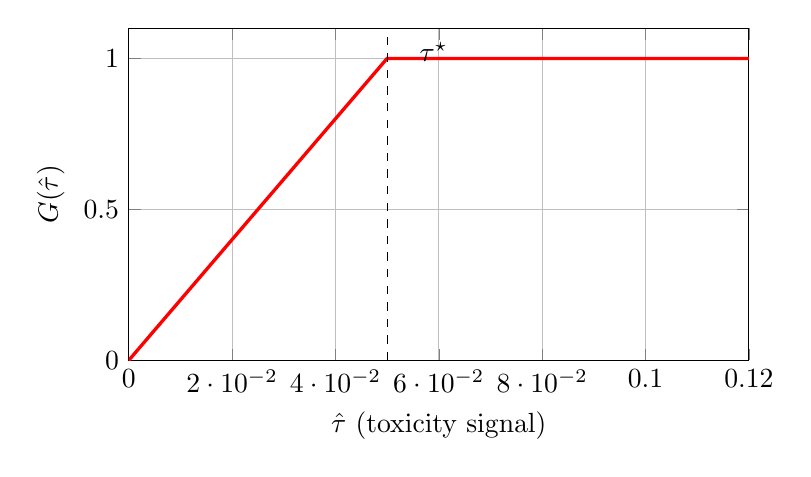
\begin{tikzpicture}
\begin{axis}[
    width=0.78\textwidth,
    height=5.8cm,
    xlabel={$\hat\tau$ (toxicity signal)},
    ylabel={$G(\hat\tau)$},
    xmin=0, xmax=0.12,
    ymin=0, ymax=1.1,
    grid=both
]
\addplot[red,very thick] coordinates {(0,0) (0.05,1) (0.12,1)};
\addplot[dashed] coordinates {(0.05,0) (0.05,1.1)};
\node at (axis cs:0.059,1.02) {$\tau^\star$};
\end{axis}
\end{tikzpicture}
\end{center}

\subsection{Hysteresis concept}
With signal $h_t$:
\begin{equation}
\text{mode}_{t+1}=
\begin{cases}
\text{PROTECT}, & \text{if mode}_t=\text{CALM and } h_t\ge T_{on},\\
\text{CALM}, & \text{if mode}_t=\text{PROTECT and } h_t\le T_{off},\\
\text{mode}_t, & \text{otherwise},
\end{cases}
\end{equation}
with $T_{off}<T_{on}$.

\begin{center}
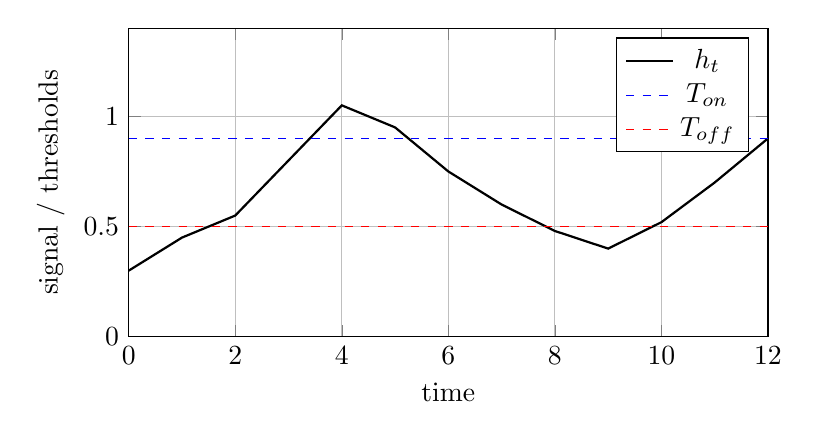
\begin{tikzpicture}
\begin{axis}[
    width=0.80\textwidth,
    height=5.5cm,
    xlabel={time},
    ylabel={signal / thresholds},
    xmin=0, xmax=12,
    ymin=0, ymax=1.4,
    grid=both,
    legend pos=north east
]
\addplot[black,thick] coordinates {
(0,0.30) (1,0.45) (2,0.55) (3,0.80) (4,1.05) (5,0.95)
(6,0.75) (7,0.60) (8,0.48) (9,0.40) (10,0.52) (11,0.70) (12,0.90)
};
\addlegendentry{$h_t$}
\addplot[blue,dashed] coordinates {(0,0.90) (12,0.90)};
\addlegendentry{$T_{on}$}
\addplot[red,dashed] coordinates {(0,0.50) (12,0.50)};
\addlegendentry{$T_{off}$}
\end{axis}
\end{tikzpicture}
\end{center}

\section{Recommended Next Formula (yq-v3 candidate)}
A compact, selective extension:
\begin{equation}
\Delta\hat\sigma_t = [\hat\sigma_t-\hat\sigma_{t-1}]_+,
\quad
u_t=\frac{\Delta\hat\sigma_t}{\max(\hat\sigma_{t-1},\epsilon)},
\quad
T_t=[u_t-\theta]_+,
\quad
G_t=\min\left(1,\frac{\hat\tau_t}{\tau^\star}\right),
\end{equation}
\begin{equation}
\Delta f_t^{protect} =
1_{\text{firstInStep}}\cdot c_m \cdot T_t \cdot G_t.
\end{equation}

Apply $\Delta f_t^{protect}$ primarily to the protect side, while retaining an attract-side calm cap:
\begin{equation}
\text{if } \hat\tau_t<\tau_{low}\ \text{and}\ a_t<a_{low},\ \text{then}\ f_{attract}\le f_N+b.
\end{equation}

This is mathematically consistent with both reports:
\begin{itemize}
    \item maximize selectivity in time (first-in-step),
    \item maximize selectivity in regime (relative surprise and toxicity gate),
    \item preserve retail competitiveness in calm states.
\end{itemize}

\section{Equation-to-Variable Mapping}
\begin{center}
\begin{tabular}{>{\ttfamily}p{2.7cm} p{10.4cm}}
\toprule
Code variable & Mathematical interpretation \\
\midrule
\texttt{pHat} & $\hat p_t$: internal fair-price estimator \\
\texttt{sigmaHat} & $\hat\sigma_t$: volatility estimate from first-in-step returns \\
\texttt{lambdaHat} & $\hat\lambda_t$: estimated trade arrivals per step \\
\texttt{sizeHat} & $\hat q_t$: normalized trade-size state \\
\texttt{toxEma} & $\hat\tau_t$: stale-price toxicity signal \\
\texttt{actEma} & $a_t$: recent activity signal \\
\texttt{dirState} & $d_t$: directional pressure around neutral center 1 \\
\texttt{stepTradeCount} & $n_t$: number of trades observed in current timestamp \\
\texttt{fBase} & base fee component from vol/arrival/flow-size \\
\texttt{fMid} & symmetric widened fee before bid/ask asymmetry \\
\texttt{skew} & direction and direction-toxicity asymmetry size \\
\bottomrule
\end{tabular}
\end{center}

\section{Final Takeaway}
\begin{itemize}
    \item \texttt{Strategy.sol} is already a strong near-frontier structure.
    \item The dominant failure mode is over-widening in low-risk states.
    \item Best next progress comes from \textbf{selective transition protection}, not globally higher fees.
\end{itemize}

\end{document}
